\documentclass{beamer}

% Some common packages
\usepackage{graphicx, color}
\usepackage{alltt}
\usepackage{booktabs, calc, rotating}
\usepackage[round]{natbib}
\usepackage{multicol}
\usepackage{amsmath, amsbsy, amssymb, amsthm, graphicx}
\usepackage[english]{babel}
\usepackage{xkeyval} 
\usepackage{xfrac}
\usepackage[normalem]{ulem}
\usepackage{fancyvrb} 
\usepackage{tikz, geometry, tkz-graph, xcolor}
\usepackage[latin1]{inputenc}
\usepackage{times}
\usepackage[T1]{fontenc}

% Shortcuts
\newcommand{\empr}[1]{{\emph{\color{red}#1}}}
\newcommand{\cov}{\mathrm{cov}}
\newcommand{\pkg}[1]{{\textbf{\texttt{#1}}}}
\newcommand{\dif}{\mathrm{d}}
\newcommand{\bigbrk}{\vspace*{2in}}
\newcommand{\smallbrk}{\vspace*{.1in}}
\newcommand{\midbrk}{\vspace*{1in}}
\newcommand{\red}[1]{{\color{red}#1}}
\newcommand{\blue}[1]{{\color{blue}#1}}
\newcommand{\green}[1]{{\color{green}#1}}
\newcommand{\calc}[1]{{\fbox{\mbox{#1}}}}
\newcommand{\Var}{\mathrm{Var}}%
\newcommand{\Cov}{\mathrm{Cov}}%

\mode<presentation>
{
	\usetheme{UTD}
	\usecolortheme[RGB={200,0,0}]{structure}
	\setbeamercovered{transparent}
}

% fancy for Verbatim?
\fvset{frame=single,framesep=1mm,fontfamily=courier,fontsize=\scriptsize,numbers=left,framerule=.3mm,numbersep=1mm,commandchars=\\\{\}}


\title[Survival Analysis]{Applied Survival Analysis Using R\\ Chapter 12: Additional Topics}
\author[Qi Guo]{Qi Guo}
\institute[UTD]{Department of Mathematical Sciences \\ 
	The University of Texas at Dallas}
\date{April, 20 2019}
	
\begin{document}

\begin{frame}
  \titlepage
\end{frame}

% Set up UTD backgroud
\setbeamercolor*{item}{fg=red}
\bgroup
\usebackgroundtemplate{
\tikz[overlay,remember picture] \node[opacity=0.05, at=(current page.center)] {
   
\includegraphics[height=\paperheight,width=\paperwidth]{UTDbg}};}


\section[Outline]{}
\begin{frame}
  \tableofcontents
\end{frame}

\section{Using Piecewise Constant Hazards to Model Survival Data}
\begin{frame}
\frametitle{What is ``\texttt{piecswise}''?}
\begin{itemize}
\item The \empr{piecewise exponential model} is a \empr{generalization} of the exponential which can offer \empr{considerable flexibility} for modeling.
\item  ``\texttt{pieces}'' means \empr{the survival time axis} was divided into multiple intervals and the \empr{hazard is constant}.
\item \empr{The piecewise exponential is that the likelihood is equivalent to a Poisson likelihood}.
\item If it is a single piece, that means it's just an ordinary exponential distribution with rate parameter $\lambda$.
\begin{equation}
L_e(\lambda) = \prod\limits_{i=1}^{n}h(t_i)^{\delta_i}S(t_i) = \prod\limits_{i=1}^{n}\lambda^{\delta_i}e^{-\lambda t_i} = \lambda^d e^{-\lambda V}
\end{equation}
where $t_i$ is the failure time of the $i$th subject, $V = \sum t_i$ is the total time at risk. 
\end{itemize}
\end{frame}

\pagebreak
\begin{frame}
\frametitle{Poisson Distribution}
\begin{itemize}
\item In Chapter 2, the m.l.e is given by $\hat{\lambda} = d/V$, now we suppose the $d$(the number of death) has a \empr{Poisson distribution} with mean $\mu$, so $\mu = V\lambda$.
\item The likelihood function for a Poisson distribution is:
\begin{equation}
L_p(\lambda) = (\lambda V)^d e^{-\lambda V} = \lambda^d e^{-\lambda V}\cdot V^d
\end{equation}
Clearly the Poisson likelihood $L_p$ is \empr{proportional} to the exponential likelihood $L_e$, the constant multiple being $V^d$
\end{itemize}
\end{frame}

\pagebreak
\begin{frame}
\frametitle{Notations}
\begin{itemize}
\item Suppose that we divide the time axis into contiguous intervals using cut points 0, $c_1$, $c_2$,..., $c_k$.
\item For each subject, say $i$, we denote the time spent in each interval by $t_{i1}$, $t_{i2}$,...,$t_{ik'}$, where $k'$ denotes the time interval subject $i$ dies, or the \empr{largest} time interval subject $i$ is still known to be alive.
\item Define $\delta_{ij}$ to be 0 for each interval $j$ in which the $i$th subject is known to be alive, and 1 for interval $k$ if the subject died in that interval.
\item Then for patient $i$, the survival time of that patient is $t_i = \sum_{j=1}^{k}t_{ij}$ and the censoring indicator is $\delta_i =\sum_{j=1}^{k}\delta_{ij}$.
\end{itemize}
\end{frame}

\pagebreak
\begin{frame}
\frametitle{Formulas}
\begin{itemize}
\item Assume a proportional hazards model
\begin{equation}
\lambda_i(t_i, \beta) = \lambda_0(t_i)e^{z_i\beta}
\end{equation}
where now the \empr{baseline hazard} is a \empr{piecewise} exponential,$\lambda_0(\mu)=\lambda_j$, $j$ being $j$th interval, the one in which $\mu$ falls, so the full likelihood is:
\begin{equation}
L_{pe}(\lambda_1, \lambda_2,...,\lambda_k,\beta) = \prod\limits_{i=1}^{n}\prod\limits_{j=1}^{k'(i)}{\lambda_{ij}}^{\delta_{ij}}e^{-\lambda_{ij} t_{ij}}
\end{equation}
where $\lambda_{ij} = \lambda_j e^{z_i\beta}$, which is the proportional hazards assumption for the piecewise exponential
\item With the single exponential, treat the censoring indicators $\delta_{ij}$ as a Poisson distribution with mean $\lambda_{ij}t_{ij}$
\end{itemize}
\end{frame}


\pagebreak
\begin{frame}
\frametitle{m.l.e}
\begin{itemize}
\item so the maximum likelihood estimates obtained from the Poisson model with
\begin{equation}
\log( \lambda_{ij}) = \log(\lambda_j) + z_i\beta = \alpha_j + z_i\beta
\end{equation}
\item so for the piecewise exponential proportional hazards model
\begin{equation}
\log( \lambda_{ij}t_{ij}) = \log(\lambda_j) + z_i\beta +\log(t_{ij})= \alpha_j + z_i\beta +\log(t_{ij})
\end{equation}
where the $\alpha_j$ are the logs of the baseline hazard coefficients and $\beta$,is the log of the hazard ratio for $z_i$, The constant log.tij/ is called an \empr{offset}.
\end{itemize}
\end{frame}

\pagebreak
\begin{frame}[fragile]
\frametitle{Example}
\begin{itemize}
\item Consider a synthetic example in Chapter 4.
\begin{Verbatim}
> tt <- c(6, 7, 10, 15, 19, 25)
> delta <- c(1, 0, 1, 1, 0, 1)
> trt <- c(0, 0, 1, 0, 1, 1)
> id <- 1:6
> simple <- data.frame(id, tt, delta, trt)
> simple
   id   tt   delta   trt 
1   1    6     1      0 
2   2    7     0      0 
3   3   10     1      1 
4   4   15     1      0 
5   5   19     0      1 
6   6   25     1      1
\end{Verbatim}
\item Define three intervals that we will use to define a piecewise exponential distribution, and partition the data into
events and person-weeks per interval:
\end{itemize}
\end{frame}

\pagebreak
\begin{frame}[fragile]
\frametitle{Example}
\begin{figure}[h!]
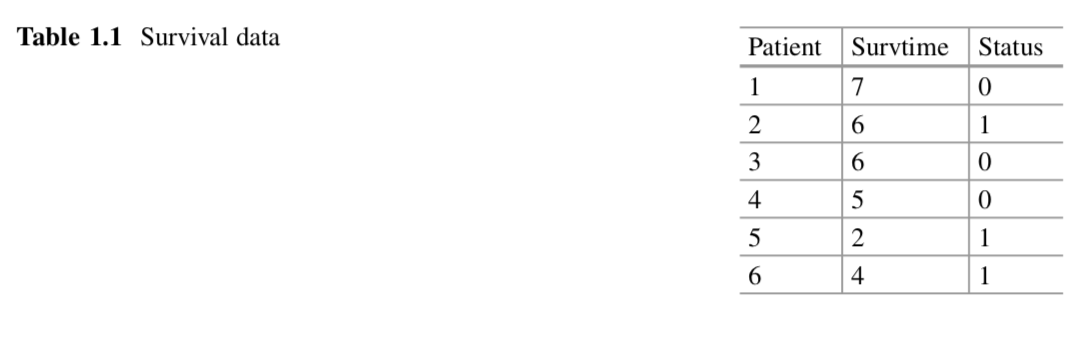
\includegraphics[scale = .3]{001.png}
\end{figure}
\begin{itemize}
\begin{Verbatim}
> tau.s <- c(0, 8, 16, 30)
> simple.split.s <- survSplit(data=simple, cut=tau.s, end="tt",
start="t0", event="delta", episode="diagGrp")
> simple.split.s$expo <- simple.split.s$tt - simple.split.s$t0
> ord <- order(simple.split.s$id)
> simple.split.ord <- simple.split.s[ord,]
> simple.split.ord
\end{Verbatim}
\end{itemize}
\end{frame}

\pagebreak
\begin{frame}[fragile]
\frametitle{Example}
\begin{itemize}
\begin{Verbatim}
    id   tt   delta   trt   t0   diagGrp   expo 
7    1    6       1     0    0         1      6 
8    2    7       0     0    0         1      7 
9    3    8       0     1    0         1      8 
15   3   10       1     1    8         2      2 
10   4    8       0     0    0         1      8 
16   4   15       1     0    8         2      7 
11   5    8       0     1    0         1      8 
17   5   16       0     1    8         2      8 
23   5   19       0     1   16         3      3 
12   6    8       0     1    0         1      8 
18   6   16       0     1    8         2      8 
24   6   25       1     1   16         3      9 
\end{Verbatim}
\item To obtain parameter estimates for the piecewise exponential distribution in (6)
\begin{Verbatim}
> result.simple.poisson <- glm(delta ~ -1 + factor(diagGrp)+trt+
offset(log(expo)), family=poisson, data=simple.split.ord)
> summary(result.simple.poisson)
\end{Verbatim}
\end{itemize}
\end{frame}

\pagebreak
\begin{frame}[fragile]
\frametitle{Example}
\begin{itemize}
\begin{Verbatim}
Coefficients:                Estimate  Std. Error  z value   Pr 
(>|z|)
factor(diagGrp)1   -3.2942   1.0370    -3.177      0.00149 **
factor(diagGrp)2   -1.7463   0.8569    -2.038      0.04156 *
factor(diagGrp)3   -1.0912   1.5949    -0.684      0.49389
trt                -1.3937   1.2425    -1.122      0.26199
---
Signif. codes:  0*** 0.001 ** 0.01 * 0.05 . 0.1    1
\end{Verbatim}
\item The ``\texttt{-1}'' in the model definition tells R to fit a separate term for each of the three interval factors (rather than to consider the first level as a reference level), more details see book!
\end{itemize}
\end{frame}

\section{Interval Censoring}
\begin{frame}
\frametitle{Right Censoring and Interval Censoring}
\begin{itemize}
\item Right censoring occurs naturally in clinical trials in Chapter 1, and  the general likelihood function:
\begin{equation}
L(\beta) = \prod\limits_{i \in D}^{}f(t_i)\cdot \prod\limits_{i \in C}^{}S(t_i)  
\end{equation}
where $D$ represents the set of all subjects who fail and $R$ the set of all who are right-censored.
\item  Suppose that some of the observations are \empr{interval-censored}, so that,patient $k$ has an event that lies between times $L_k$ and $R_k$.
\begin{equation}
L(\beta) = \prod\limits_{i \in D}^{}f(t_i)\cdot \prod\limits_{i \in C}^{}[S(t_i) - S(R_i)]  
\end{equation}
\end{itemize}
\end{frame}

\pagebreak
\begin{frame}
\frametitle{Example}
\begin{itemize}
\item If an event is only known to have occurred before a particular time $R_i$, this is known as \empr{left censoring}, and accommodated by setting $L_i = 0$
\item A special optimization technique known as the \empr{Expectation
-Maximization algorithm} to get m.l.e.
\begin{problock}{Breast Cosmesis Study}
Fit a proportional hazards model to interval-censored data, and illustrated it using data from a breast cosmesis study. In this study, 94 breast cancer patients treated with radiation therapy with or without adjuvant chemotherapy were followed to determine the time until cosmetic deterioration (specifically, the appearance breast retraction) of the treated breast. Since patients were evaluated at office visits separated by a number of months, the data were interval-censored.
\end{problock}
\end{itemize}
\end{frame}

\pagebreak
\begin{frame}[fragile]
\frametitle{Example}
\begin{itemize}
\begin{Verbatim}
> library(interval)
> data(bcos)
> bcos[c(1,33, 47, 62, 90),]
       left    right    treatment 
1       45       Inf          Rad 
33       0         5          Rad 
47       8        12      RadChem 
62      14        17      RadChem
90      16        60      RadChem
\end{Verbatim}
\item  Patient 47 received radiation and adjuvant chemotherapy, had not had the event at an office visit at 8 months, but the breast retraction had been observed at the next visit four months later. Thus, the event took place sometime between 8 and 12 months
\end{itemize}
\end{frame}

\pagebreak
\begin{frame}[fragile]
\frametitle{Example}
\begin{itemize}
\item obtain m.l.e of the survival distributions and plot:
\begin{Verbatim}
> icout <- icfit(Surv(left,right,type="interval2")~treatment,
data=bcos, conf.int=F)
> plot(icout, XLAB="Time in months", YLAB="Survival probability", 
COL=c("lightblue", "pink"), LEGEND=F, estpar=list(col=
c("blue", "red"), lwd=2, lty=1))
> legend("bottomleft",legend=c("Radiation alone", "Radiation and 
chemo"), col=c("blue","red"), lwd=2)
\end{Verbatim}
\item fit a Weibull proportional hazards model to the interval-censored data, first we must define modified left and right endpoints of the intervals and set a maximum possible time.
\end{itemize}
\end{frame}

\pagebreak
\begin{frame}[fragile]
\frametitle{Example}
\begin{itemize}
\begin{Verbatim}
> bcos <- within(bcos, \{
left.alt <- left
left.alt[left == 0] <- 0.1
right.alt <- right
right.alt[is.infinite(right)] <- 65\})
> bcos[c(1,33, 47, 62, 90),]
       left    right    treatment    right.alt    left.alt
1       45       Inf          Rad           65        45.0
33       0         5          Rad            5         0.1
47       8        12      RadChem           12         8.0
62      14        17      RadChem           17        14.0
90      16        60      RadChem           60        16.0
\end{Verbatim}
\item fit the Weibull model and add the fitted survival curves as follows:
\end{itemize}
\end{frame}

\pagebreak
\begin{frame}[fragile]
\frametitle{Example}
\begin{figure}[h!]
\includegraphics[scale = .25]{006.png}
\end{figure}
\begin{Verbatim}
> bcos.survreg <-survreg(Surv(left.alt, right.alt, type="interval2") ~ 
treatment, dist="weibull", data=bcos)
> pct <- 1:999/1000
> ptime <- predict(bcos.survreg, type='quantile',
newdata=data.frame(treatment=c("Rad", "RadChem")),p=pct, se=F)
> ines(ptime[1,], 1-pct, xlab="Hours", ylab="Survival", type='l',
lty=c(1,2,2), lwd=c(2,1,1), xlim=c(0,20), col="blue") 
> lines(ptime[2,], 1-pct, xlab="Hours", ylab="Survival", type='l',
lty=c(1,2,2), lwd=c(2,1,1), xlim=c(0,20), col="red")
\end{Verbatim}
\end{frame}


\section{The Lasso Method for Selecting Predictive Biomarkers}
\begin{frame}
\frametitle{select covariates}
\begin{itemize}
\item In some applications, by contrast, our interest focuses on the predictive ability of a set of covariates. the biomarker focus on using those measurements to \empr{predict} a patient's survival prospects.
\item An important such method is the ``\texttt{lasso}'' procedure  in the R package ``\texttt{penalized}'' 
\item This approach \empr{maximizes} the partial likelihood function $\ell(\beta) = \log L(\beta)$
\begin{equation}
L(\beta) = \prod\limits_{j=1}^{D} \frac{h_0(t_j)\psi_j}{\sum\limits_{k\in R_j}^{}h_0(t_j)\psi_k} = \prod\limits_{j=1}^{D}\frac{\psi_j}{\sum\limits_{k \in R_j}^{}\psi_k}
\end{equation}
\end{itemize}
\end{frame}

\pagebreak
\begin{frame}
\frametitle{lasso procedure}
\begin{itemize}
\item The parameter satisfies the \empr{constraint} $\sum_{j=1}^{p}|\beta_j|\le t$ for a constant $t$, where $p$ is the number of parameters,this may be shown to be equivalent to maximizing the penalized likelihood which, for a pre-specified value of $\lambda$.
\begin{equation}
\ell_{pen}(\beta) = \ell(\beta) - \lambda \sum\limits_{j=1}^{p}|\beta_j|
\end{equation}
\item A sufficiently large value of $\lambda$ will result in \empr{no covariates} at all in the model, and smaller $\lambda$ values will cause non-zero coefficient estimates.
\item How do we select $\lambda$?
\end{itemize}
\end{frame}

\pagebreak
\begin{frame}
\frametitle{Cross Validation}
\begin{itemize}
\item The goal of the procedure is \empr{accurate prediction}, to add the predictive accuracy, we have a procedure called \empr{cross validation}.
\item Cross Validation:
\begin{itemize}
\item Start with an initial value of $\lambda$ and randomly divide the data set into \empr{five} subsets of approximately equal size.
\item Select one of the subsets to be what we shall call the ``\texttt{validation}'' set(20\%), and combine the remaining subsets into what we shall call the ``\texttt{training}'' set(80\%).
\item Use the training set to construct the lasso model based on (10), and use this model to predict the survivals of patients in the validation set.
\end{itemize}
\end{itemize}
\end{frame}

\pagebreak
\begin{frame}
\frametitle{Cross Validation}
\begin{itemize}
\item Use a partial-likelihood-based measure of goodness-of-fit to these data.
\item \empr{Repeat} this four more times, with each of the remaining four subsets in turn playing the role of the 20\% validation set and the others being the training set.
\item Derive an \empr{average} partial-likelihood goodness of fit, and  repeated for a range of values of $\lambda$, and we select that value that produces the \empr{optimum} goodness of fit.
\end{itemize}
\end{frame}

\pagebreak
\begin{frame}[fragile]
\frametitle{Example}
\begin{problock}{Example 2}
The data contains 17 clinical and biomarker measurements on 227 patients, as well as overall survival and time to recurrence, both recorded in months. Of the 227 patients, 117 have levels of a variety of chemokines and other markers, some representing levels in the tumor itself and some outside the tumor, use 26 of these measurements (columns 23 to 48) as potential predictors of overall survival using a lasso model
\end{problock}
\begin{itemize}
\item Selecting the 117 patients with complete data:
\begin{Verbatim}
hepatoCellularNoMissing<-hepatoCellular[
complete.cases(hepatoCellular),]
\end{Verbatim}
\end{itemize}
\end{frame}

\pagebreak
\begin{frame}[fragile]
\frametitle{Example}
\begin{itemize}
\item ``\texttt{OS}'' (overall survival), ``\texttt{Death}''(censoring) and a few of the cytokine measurements
\begin{Verbatim}
> hepatoCellularNoMissing[c(1,5,12),c(16,17, 23:27)]
    OS Death      CD4T       CD4N       CD8T     CD8N       CD20T
1   83     0  2.600000   0.000000   190.6000   126.80   20.950000 
76  20     1 14.450000   2.758621     2.1500    38.95   26.100000
131 35     1  2.821133   8.294828     8.0064    62.64    2.821133
\end{Verbatim}
\item Then we fit a simple lasso model using the 26 predictors (columns 23 to 48), and we fix the penalty at $\lambda = 10$.
\begin{Verbatim}
> attach(hepatoCellularNoMissing)
> library(penalized)
> hepato.pen <- penalized(Surv(OS,Death),
penalized=hepatoCellularNoMissing[,23:48],
standardize=T, lambda1=10) # nonzero coefficients: 7
\end{Verbatim}
\end{itemize}
\end{frame}

\pagebreak
\begin{frame}[fragile]
\frametitle{Example}
\begin{itemize}
\item List their values using the ``\texttt{coef}'' function
\begin{Verbatim}
> round(coef(hepato.pen, standardize=T), 3)
 CD8N  CD68T    CD4TR    CD8TR   CD68TR    Ki67    CD34 
0.104  0.258   -0.035   -0.096    0.111   0.285  -0.013
\end{Verbatim}
\item Use cross- validation to select a value that optimizes the predictive ability of the lasso model, as defined by maximizing the cross-validated partial log-likelihood(CVL).
\begin{Verbatim}
> set.seed(34)
> hepato.prof <- profL1(Surv(OS, Death),
penalized=hepatoCellularNoMissing[,23:48],
standardize=T, fold=10, minlambda1=2, maxlambda1=12)
> plot(hepato.prof$cvl ~ hepato.prof$lambda, type="l", log="x",
xlab="lambda", ylab="Cross-validated log partial likelihood")
\end{Verbatim}
\item ``\texttt{set.seed}''  is to set the random number seed so that we can reproduce this model fit exactly.
\end{itemize}
\end{frame}

\pagebreak
\begin{frame}[fragile]
\frametitle{Example}
\begin{itemize}
\item To find the optimal value, we use ``\texttt{OptL1}'' with the same starting seed.
\begin{Verbatim}
> set.seed(34)
> hepato.opt <- optL1(Surv(OS, Death),
penalized=hepatoCellularNoMissing[,23:48], standardize=T,
fold=10)
> hepato.opt$lambda
[1] 8.242321
> abline(v=hepato.opt$lambda, col="gray")
\end{Verbatim}
\item The optimal value is 8.24.
\end{itemize}
\end{frame}

\pagebreak
\begin{frame}
\frametitle{Example}
\begin{figure}[h!]
\includegraphics[scale = .45]{007.png}
\end{figure}
\end{frame}
\end{document}